\section{Unifying DM and SHM}
\label{sec:hadm}

This section discusses the benefits of a unified DM/SHM approach and outlines some of the key implementation details.

\subsection{Separated vs. unified DM/SHM}

The next example illustrates how unification can be helpful in balancing system health needs and operational objectives:

\begin{figure}[h]
	\centering
		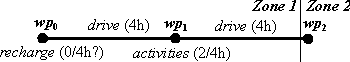
\includegraphics[width=0.85\columnwidth]{figures/shm_dm_example.pdf}
	\caption{Separated vs. unified DM/SHM (Example \ref{ex:separated_unified})}
	\label{fig:shm_dm_example}
\end{figure}

\begin{figure}[h]
	\centering
		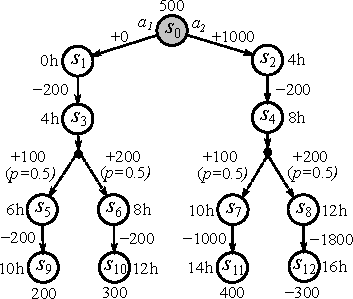
\includegraphics[width=0.75\columnwidth]{figures/shm_dm_tree_compact.pdf}
	\caption{Execution scenarios in Example \ref{ex:separated_unified}}
	\label{fig:shm_dm_tree}
\end{figure}

%\begin{itemize}
\begin{ex}
\label{ex:separated_unified}
The rover starts at $wp_0$ in Zone 1 (Figure \ref{fig:shm_dm_example}) with $\unit[500]{Wh}$ in the battery (out of the $\unit[1500]{Wh}$ capacity). The solar panels can charge the battery at a rate of $\unit[250]{W}$. Sunlight in Zone 1 will last for another 12 hours.

Two actions are available in the initial state $s_0$ at $wp_0$ (Figure \ref{fig:shm_dm_tree}): skip charging ($a_1 = + \unit[0]{Wh}$) and charge to full ($a_2 = + \unit[1000]{Wh}$). In Figure \ref{fig:shm_dm_tree}, the unitless numbers are Watt-hours of energy going in or out of the battery. Time (in hours) at each state is denoted as '$\unit[\text{[t]}]{\text{h}}$'.

The rover needs to perform a 2-hour stationary science activity at $wp_1$ and be able to arrive at $wp_2$, the next recharge point. The prior probability of the activity at $wp_1$ needing to be redone (a 2-hour delay) is $0.5$. Science payload power consumption is $\unit[100]{W}$, resulting in a net-positive ($\unit[250]{W} -\unit[200]{W} = +\unit[50]{W}$) power flow.

The driving times from $wp_0$ to $wp_1$ and from $wp_1$ to $wp_2$ are $4$ hours, with the average drive train power consumption of $\unit[300]{W}$, resulting in a net-negative ($\unit[250]{W} -\unit[300]{W} = -\unit[50]{W}$) power flow.

If operating without sunlight, a $\unit[150]{W}$ heater needs to be used to keep batteries and electronics warm, thus resulting in a net-negative power flow of $-\unit[300]{W} -\unit[150]{W} = - \unit[450]{W}$ for driving and $- \unit[200]{W} - \unit[150]{W} = - \unit[350]{W}$ for stationary science activities.
\end{ex}

According to the general SHM policy of restoring health (battery charge, in this case) to nominal, the action chosen at $wp_0$ is $\pi_{shm}(s_0) = a_2$ and the battery is recharged to full $\unit[1500]{Wh}$. After the science activity at $w_1$ is completed, assessment is made that it needs to be repeated. The 2-hour delay means that the entirety of $wp_1 \rightarrow wp_2$ segment needs to be done without sunlight, resulting in a complete battery depletion before $wp_2$ is reached, with a deficit of $\unit[300]{Wh}$.

In computing a unified policy, however, where SHM actions are considered in the context of the overall mission, all four scenarios depicted in Figure \ref{fig:shm_dm_tree} would play a role. The expected amount of battery charge remaining if $a_1$ is chosen would be $Q_1 = 0.5 \cdot 200 + 0.5 \cdot 300 = 250$. For $a_2$: $Q_2 = 0.5 \cdot 400 + 0.5 \cdot (-300) = 50$. Action $a_1$ (no recharge) would be chosen and, with the two-hour delay at $wp_1$, the rover would arrive at $wp_2$ with $\unit[300]{Wh}$ still remaining.

The example illustrates the first benefit of unifying DM and SHM: the ability to naturally take operational objectives and constraints into account when making a system health recovery decision. The next example illustrates how DM, on the other hand, can benefit from unified action spaces and access to health-related models:

\begin{figure}[h]
	\centering
		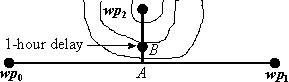
\includegraphics[width=0.7\columnwidth]{figures/action_spaces_example_compact.pdf}
	\caption{Unified action spaces (Example \ref{ex:action_spaces})}
	\label{fig:action_spaces}
\end{figure}

\begin{ex}
\label{ex:action_spaces}

The rover is traveling from $wp_0$ to $wp_1$ (flat terrain) when a decision is made at point A to make a detour and attempt data collection at a scientifically valuable $wp_2$, requiring a 6-hour climb up a steep hill (Figure \ref{fig:action_spaces}). The 1-hour data collection activity at $wp_2$ must be completed before the loss of illumination there in $10$ hours. 
	
After completing the 2-hour climb up to point $B$ ($1/3$ of the way up), it is observed that the internal temperature of one of the drive motors has risen to $T_m=\unit[60^\circ]{C}$ from the nominal of $\unit[20^\circ]{C}$. At $T_m=\unit[80^\circ]{C}$ there is a significant risk of permanent damage and failure of the motor.
\end{ex}

If the SHM system on the rover consists of the traditional fault detection, diagnosis, and mitigation/recovery components only, it may diagnose the fault to be \textit{increased friction}, mark the component (motor) as faulty, and set a constraint on terrain types to either \textit{flat} or \textit{downhill}. It would then invoke the recommended action for this fault from $A_\text{SHM}$: \textit{stop and cool down} (until $T_m=\unit[20^\circ]{C}$). 

If a prognostic component is present, it may predict that at the current temperature increase rate, the RUL of the motor is 1 hour (with 4 hours of climb remaining to reach $wp_2$). The same mitigation action (\textit{stop and cool down}) would be initiated and the same constraint on the current to the motor (and, thus, on the incline angle) may be set. After $T_m$ returns to nominal (which happens to take 1 hour), control is returned to DM. Based on the new constraints and the motor marked as faulty, DM would command the rover to abort the detour, return to $A$, and resume the drive to $wp_2$.

If, however, DM had \textit{stop and cool down} as part of its action space ($A_\text{DM}$) and updated the state variables for the affected motor with the newly computed heat-up and cool down rates, an operational policy could be computed that optimizes the duration of driving and cool down intervals and allows the rover to reach $wp_2$ in time. For instance, if the rover drives for two hours, then stops for an hour to cool down the motor, it can still reach $wp_2$ in $2+1+2+1+2 = 8$ hours. With the science activity taking 1 hour, there would still be an hour in reserve before the loss of sunlight at $wp_2$.

\subsection{Unification approach}
In proposing the unified DM/SHM approach, we rely heavily on \textit{utility theory} \cite{Fishburn1970}. The following, in our opinion, are the key ingredients for a successful  unification: (1) a state-based system modeling framework and (2) a utility (value) function capturing the operational preferences for the system. A \textbf{utility function} (denoted as $U$) captures, numerically, our preferences over the space of possible outcomes. For instance, we may assign a higher utility value to a rover state where a desired scientific location has been reached. Utility can be defined for system states or for state-action pairs. If, in some system state $s$, the outcome of an action $a$ (a particular state $s'$) is not guaranteed, then the \textit{expected utility} of the $(s,a)$ tuple is
\begin{equation}
U(s,a) = \sum_{s'}T(s',a,s)U(s').
\end{equation}

In a strictly deterministic system, where a plan $\{a_{0:H}\}$ up to a horizon $H$ can be provided ahead of time, the expected utility of $s$ relative to the plan is:
\begin{equation}
U^{a_{0:H}}(s) = \sum_{i=0:H}R(s_i,a_i).
\label{eq:plan}
\end{equation}
For systems with action outcome uncertainty, the expected utility associated with executing a policy $\pi$ for $t$ steps from state $s$ can be computed recursively as
\begin{equation}
U_t^{\pi}(s)=R(s,\pi(s))+\gamma \sum_{s'} T(s,\pi(s),s')U^{\pi}_{t-1}(s'),
\label{eq:U(s)}
\end{equation}
where $\gamma \in [0,1]$ is the discount factor that is sometimes used to bias towards earlier rewards, particularly in \textit{infinite horizon} problems ($t \rightarrow \infty$). The optimal utility for a state can then also be computed recursively using
\begin{equation}
U_t^*(s)=\max_{a \in A} (R(s,a)+\gamma \sum_{s'} T(s,a,s')U^*_{t-1}(s')),
\label{eq:U*(s)}
\end{equation}
which for $t \rightarrow \infty$ becomes the \textit{Bellman equation} \cite{Bellman1957}. Knowing the optimal utility function, we can derive an optimal policy:
\begin{equation}
\pi^*(s) = \argmax_{a \in A} (R(s,a)+\gamma \sum_{s'} T(s,a,s')U^*(s')).
\label{eq:pi*(s)}
\end{equation}

In problems with state uncertainty, beliefs $b \in B$ can take the place of states in equations \ref{eq:U(s)}--\ref{eq:pi*(s)} \cite{Kaelbling1998}. The \textit{Markov property} is assumed, meaning that $T(s,a,s')$ does not depend on the sequence of transitions that led to $s$ \cite{Kemeny1983}.

Now that the foundational concepts have been described, we will focus on those most relevant to the proposed unification: states and the reward function $R(s,a)$. States can be vector quantities (Section \ref{sec:systems}). For real-world problems, the relevant elements of the operating environment are sometimes included in the state vector, either explicitly or implicitly \cite{Ragi2014}. For instance, the rover state vector would certainly need to include the rover's $x$ and $y$ coordinates, but may also include time $t$. These three elements allow us to indirectly access other information about the environment, \textit{e.g.}, solar illumination, ambient temperature, communications coverage, and terrain properties.

Similarly, health-related elements can be included in the same state vector. For the rover, the battery charge would likely be in it already for operational purposes. Adding battery temperature, however, would allow for better reasoning about the state of battery health, when combined with information on ambient temperature, terrain, and recharge current. Thus, including even a few health-related elements in the state vector may have a multiplicative effect on the amount of information available. The resulting size of the state vector may also end up being smaller than the sum of separately maintained DM and SHM state vectors, as redundant elements are eliminated.

The reward function $R(s,a)$ encodes the costs and the rewards of being in a particular state or taking a particular action in a state and can also be thought of as a local utility function. For many realistic problems with multi-variable state representations, the reward function needs to combine costs or rewards pertinent to state components. Several approaches have been proposed \cite{Keeney1993}, with additive decomposition being an effective option in many cases. However it is implemented, the key property of the function is that by mapping multiple variables to a single number, it allows us to compute $U(s)$ or $U(s,a)$ and translate a potentially complex DM formulation into an abstract utility maximization problem.

As an example of such mapping, consider two different rover states: $s_1$, where the rate of battery discharge is higher than nominal due to a parasitic load in the electrical system and $s_2$, where the rover is healthy, but is traversing difficult terrain, thus also leading to a higher rate of battery discharge. The utilities $U(s_1)$ and $U(s_2)$ may end up being approximately equal, however, given the similar impact of the two issues on future rewards. Policies computed for $s_1$, $s_2$, and their follow-on states may be similar also and, for instance, could result in more frequent recharge stops.

One notable consequence of health-related components being integrated into a common state vector is that from the computational point of view the concepts of \textbf{fault} and \textbf{failure} become somewhat superfluous. If subsets $S_\text{fault} \subset S$ or $S_\text{failure} \subset S$ are defined for the system, the framework described above will not do anything differently for them. The only essential subset of $S$ is $S_T$ (the terminal states). Failure states may be part of $S_T$ if they result in termination of system operations; however, goal (success states) are members of $S_T$ also. The only difference between them is in their $U(s)$ values. As long as a component fault or a failure does not lead to a transition to a terminal state, actions that maximize the expected value of that state will be selected (which, as it happens, implements the ``fail operational'' philosophy).

\begin{figure*}[htb]
	\centering
		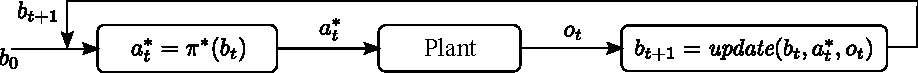
\includegraphics[width=0.7\textwidth]{figures/ops_loop.pdf}
	\caption{The main loop of health-aware decision making}
	\label{fig:ops_loop}
\end{figure*}

We will refer to this unified approach as \textbf{health-aware decision making (HADM)}. The rest of the major SHM concepts are incorporated into the new approach as follows. \textbf{Fault detection} and \textbf{diagnostics} are subsumed in belief estimation and updating, although these operations are, of course, used for nominal belief states as well. \textbf{Uncertainty management} can now be purposefully incorporated into the decision making process by either augmenting $A$ with information gathering actions \cite{Spaan2015}, evaluated in the same context as other types of actions, or by continuing to improve $U(s)$ or $U(s,a)$ estimates until a desired level of confidence in them is reached \cite{Browne2012}. For actively controlled systems, \textbf{predictive} simulations are simply an integral part of $U(s)$ calculation, where $T(s,a,s')$ serves as a one-step ``prognostic'' function (with degradation models, if any). Whereas prognostic algorithms applied to controlled systems are limited in their predictive ability due to the lack of knowledge about future actions, here the $U(s)$ calculation process is an exploration of possible execution scenarios, thus combining $s'$ or $b'$ estimation with sequential action selection.

The overall HADM operational loop (assuming state and outcome uncertainty) can be seen in Figure \ref{fig:ops_loop}. Once the initial belief $b_0$ is estimated at time $t_0$, either an offline policy is referenced or an online policy is computed to determine $a_0^*$ (best action). The action is executed by the plant, transitioning to a new (hidden) state, and generating an observation $o_0$. The observation is then used to update $b_0$ (typically through some form of Bayesian updating) and the process repeats until a terminal state is believed to be reached.

A detailed discussion of the actual algorithms that can implement the proposed approach is left for future publications, however examples of DM algorithms that can deal with state or outcome uncertainty are provided by \citeauthor{Kochenderfer2015} \shortcite{Kochenderfer2015}. In systems where both state and outcome uncertainty are not a factor, a variety of traditional state space planning algorithms \cite{Ghallab2016} would not need any modification to produce plans for spaces of state vectors that include health-related components.

\subsection{Emergency response vs. health management}

For realistic complex systems operating in the presence of state and outcome uncertainty, $S$, $B$, and $O$ are likely to be infinitely large (with $|A| \ll \infty$, although still potentially large). The problem of finding exact optimal policies in such cases is PSPACE-complete \cite{Papadimitriou1987}. Approximate solution methods typically work \textit{online}, constructing $\pi$ for the current belief $b$ based on beliefs reachable from $b$ within the decision horizon \cite{Browne2012}. They also typically perform targeted sampling from $S/B$, $A$, and $O$, thus optimality guarantees can be harder to provide. We, therefore, propose the following:
%
\begin{itemize}
	\item That \textbf{system emergency response (SER)} be defined as an automated or semi-automated process that is invoked to maximize the likelihood of preserving the system's integrity, regardless of the effect on operational goals (\textit{i.e.}, a different objective from HADM).
	\item That emergency response policy $\pi_\text{SER}$ be computed separately from the HADM policy.
\end{itemize}
%
In the space domain, an example of SER is putting a spacecraft in a \textit{safe mode} until the emergency is resolved \cite{Rasmussen2008}. In aviation, it could be executing recommendations of a collision avoidance system \cite{Kochenderfer2015}. Introduction of a separate SER system would likely require the introduction of $S_\text{SER}$, an additional $S$ subset which defines for which states $\pi_\text{SER}$ is invoked versus $\pi_\text{HADM}$. Once again, however, $S_\text{SER}$ will not necessarily only contain system fault and failure states. For instance, states where environmental conditions warrant emergency response (\textit{e.g.}, solar activity interrupting teleoperation of the rover) would be included as well. Since the scope of the SER problem is likely to be much narrower than that of HADM, it opens up the possibility of computing, verifying, and validating $\pi_\text{SER}$ \textit{offline} \cite{Kochenderfer2015}.

As sensors, computing capabilities, and DM algorithms improve further, the fraction of the system's state space that is under the purview of SER will decrease. Still, we foresee the need for a ``safety net'' SER to be there for safety-critical functions and thus advocate SER independence. SER would cover the situations where the primary HADM system may not be able to produce a suitable solution in a desired amount of time, serving as an equivalent of human reflexive responses triggered by important stimuli versus the more deliberative cognitive functionality of the brain. It could also provide dissimilar redundancy for critical regions of $S$, essentially implementing the Swiss Cheese Model \cite{Reason1990a}, which advocates multiple different layers of protection for important functions.

\subsection{Remarks on computational complexity}

A counter-argument to the unified approach can be made that it increases the computational complexity by operating on larger $S/B$, $A$, and $O$ spaces. While this is indeed a concern, algorithms have been developed in the recent years that can effectively accommodate much of the complexity, even for problems with state and outcome uncertainty, by approximating optimal policies online \cite{Silver2010,Browne2012}. Secondly, some of the complexity is removed from HADM into an independent SER component, making the former problem easier. Finally, as noted above, unifying the SHM and DM elements may also result in reduction of overlapping model variables.
